\newif\ifshowsolutions
\showsolutionstrue
\documentclass{article}
\usepackage{listings}
\usepackage{amsmath}
%\usepackage{subfigure}
\usepackage{subfig}
\usepackage{amsthm}
\usepackage{amsmath}
\usepackage{amssymb}
\usepackage{graphicx}
\usepackage{mdwlist}
\usepackage[colorlinks=true]{hyperref}
\usepackage{geometry}
\usepackage{titlesec}
\geometry{margin=1in}
\geometry{headheight=2in}
\geometry{top=2in}
\usepackage{palatino}
\usepackage{mathrsfs}
\usepackage{fancyhdr}
\usepackage{paralist}
\usepackage{todonotes}
\setlength{\marginparwidth}{2.15cm}
\usepackage{tikz}
\usetikzlibrary{positioning,shapes,backgrounds}
\usepackage{float} % Place figures where you ACTUALLY want it
\usepackage{comment} % a hack to toggle sections
\usepackage{ifthen}
\usepackage{mdframed}
\usepackage{verbatim}
\usepackage[strings]{underscore}
\usepackage{listings}
\usepackage{bbm}
\rhead{}
\lhead{}

\renewcommand{\baselinestretch}{1.15}

% Shortcuts for commonly used operators
\newcommand{\E}{\mathbb{E}}
\newcommand{\Var}{\operatorname{Var}}
\newcommand{\Cov}{\operatorname{Cov}}
\newcommand{\Bias}{\operatorname{Bias}}
\DeclareMathOperator{\argmin}{arg\,min}
\DeclareMathOperator{\argmax}{arg\,max}

% do not number subsection and below
\setcounter{secnumdepth}{1}

% custom format subsection
\titleformat*{\subsection}{\large\bfseries}

% set up the \question shortcut
\newcounter{question}[section]
\newenvironment{question}[1][]
  {\refstepcounter{question}\par\addvspace{1em}\textbf{Question~\Alph{question}\!
    \ifthenelse{\equal{#1}{}}{}{ [#1 points]}: }}
    {\par\vspace{\baselineskip}}

\newcounter{subquestion}[question]
\newenvironment{subquestion}[1][]
  {\refstepcounter{subquestion}\par\medskip\textbf{\roman{subquestion}.\!
    \ifthenelse{\equal{#1}{}}{}{ [#1 points]:}} }
  {\par\addvspace{\baselineskip}}

\titlespacing\section{0pt}{12pt plus 2pt minus 2pt}{0pt plus 2pt minus 2pt}
\titlespacing\subsection{0pt}{12pt plus 4pt minus 2pt}{0pt plus 2pt minus 2pt}
\titlespacing\subsubsection{0pt}{12pt plus 4pt minus 2pt}{0pt plus 2pt minus 2pt}


\newenvironment{hint}[1][]
  {\begin{em}\textbf{Hint: }}{\end{em}}

\ifshowsolutions
  \newenvironment{solution}[1][]
    {\par\medskip \begin{mdframed}\textbf{Solution~\Alph{question}#1:} \begin{em}}
    {\end{em}\medskip\end{mdframed}\medskip}
  \newenvironment{subsolution}[1][]
    {\par\medskip \begin{mdframed}\textbf{Solution~\Alph{question}#1.\roman{subquestion}:} \begin{em}}
    {\end{em}\medskip\end{mdframed}\medskip}
\else
  \excludecomment{solution}
  \excludecomment{subsolution}
\fi

\newcommand{\boldline}[1]{\underline{\textbf{#1}}}

% User packages
\usepackage[labelfont=bf]{caption}
\usepackage[labelfont=bf]{caption}
\usepackage[labelfont=bf]{caption}
\usepackage [english]{babel}
\usepackage [autostyle, english = american]{csquotes}
\MakeOuterQuote{"}

% User commands
\setlength{\parindent}{0pt}

\chead{%
  {\vbox{%
      \vspace{2mm}
      \large
      Machine Learning \& Data Mining \hfill
      Caltech CS/CNS/EE 155 \hfill \\[1pt]
      Miniproject 1\hfill
      Released January $28^{th}$, 2017 
    }
  }
}

\begin{document}
\pagestyle{fancy}

\section*{1. Introduction}
\medskip
\begin{itemize}

    \item \boldline{Group members} \\
    Eli Sorey \\
    Kun ho (John) Kim 
    
    \item \boldline{Team name} \\
    Stochastic Gradient, Decent
    
    \item \boldline{Division of labour} \\
    Eli focused on dataset cleaning, feature selection, and feature transformation. (Feature Engineering) Kun ho primarily worked on the model 
    selection, model parameter optimization, and ensemble selection methods. (Models and techniques) We delve into the specific of our work in the following sections.

\end{itemize}



\section*{2. Overview}
\medskip
\begin{itemize}

    \item \boldline{Models and techniques tried}
    \begin{itemize}
    \item \textbf{*Ensemble Selection:} Submitted model. 
    \item \textbf{Gradient Boosting Machines} 
    \item \textbf{Random Forest} 
    \item \textbf{Adaptive Boosting} 
    \item \textbf{Extra Trees} 
    \item \textbf{Support Vector Machines} 
    \item \textbf{Artificial Neural Networks} 
    \end{itemize}

    \item \boldline{Work timeline}
    \begin{itemize}
    \item \textbf{Day1 - Day4:} Preliminary data-processing \& Broad model selection. 
    \item \textbf{Day 4 - Day 8:} Feature engineering \& Single model optimization
    \item \textbf{Day 8 - Day 12:} Ensemble selection \& Final model tuning
    \end{itemize}

\end{itemize}


\newpage


\section*{3. Approach \& Results}
\subsection*{3.1. Overview}
Our team's general pipeline for this competition is outlined in the flow chart below. \\
\begin{figure}[h]
\center
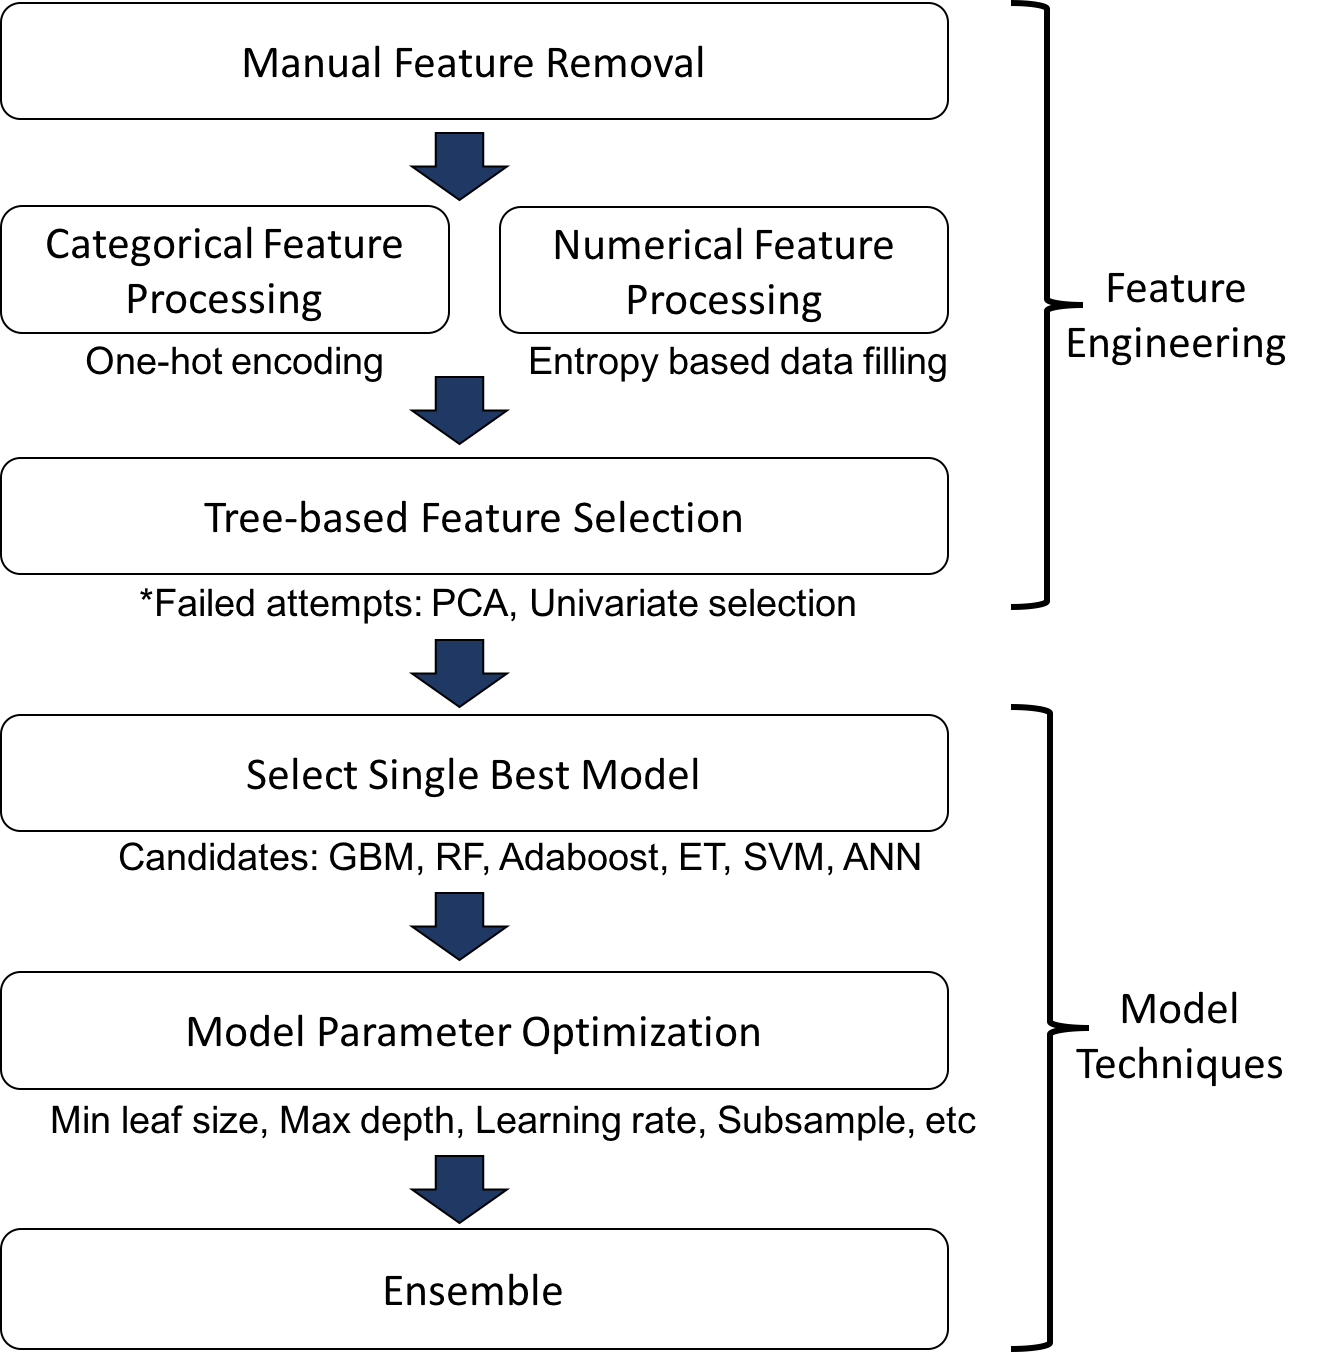
\includegraphics[scale=0.4]{figure1/figure1.png}
\caption{\textbf{Overall pipeline}}
\end{figure}

We first sought to transform the raw training data into a compact representation while keeping all the relevant information. The feature engineering part of the workflow covers methods of handling categorical features, numerical features, and the feature selection process. The model \& techniques part covers our methods of model selection, parameter 
optimization, and stacking/ensemble selecting single models. 

\subsection*{3.2. Feature engineering}


\newpage

\subsection*{3.3. Model \& Techniques}
\subsubsection*{[i]. Single model selection through cross validation}
After preprocessing the training data, 6 broad model classes(GBM, RF, Adaboost, ET, SVM, ANN) were considered as candidates to determine which achieves the best single-model performance. 5-fold cross validation was performed and the model with the highest validation accuracy was chosen. The following bar graph demonstrates that gradient boosting machines (GBM) performed the best with a validation accuracy of $77.9\%$ (with default parameters). 
\begin{figure}[h]
\center
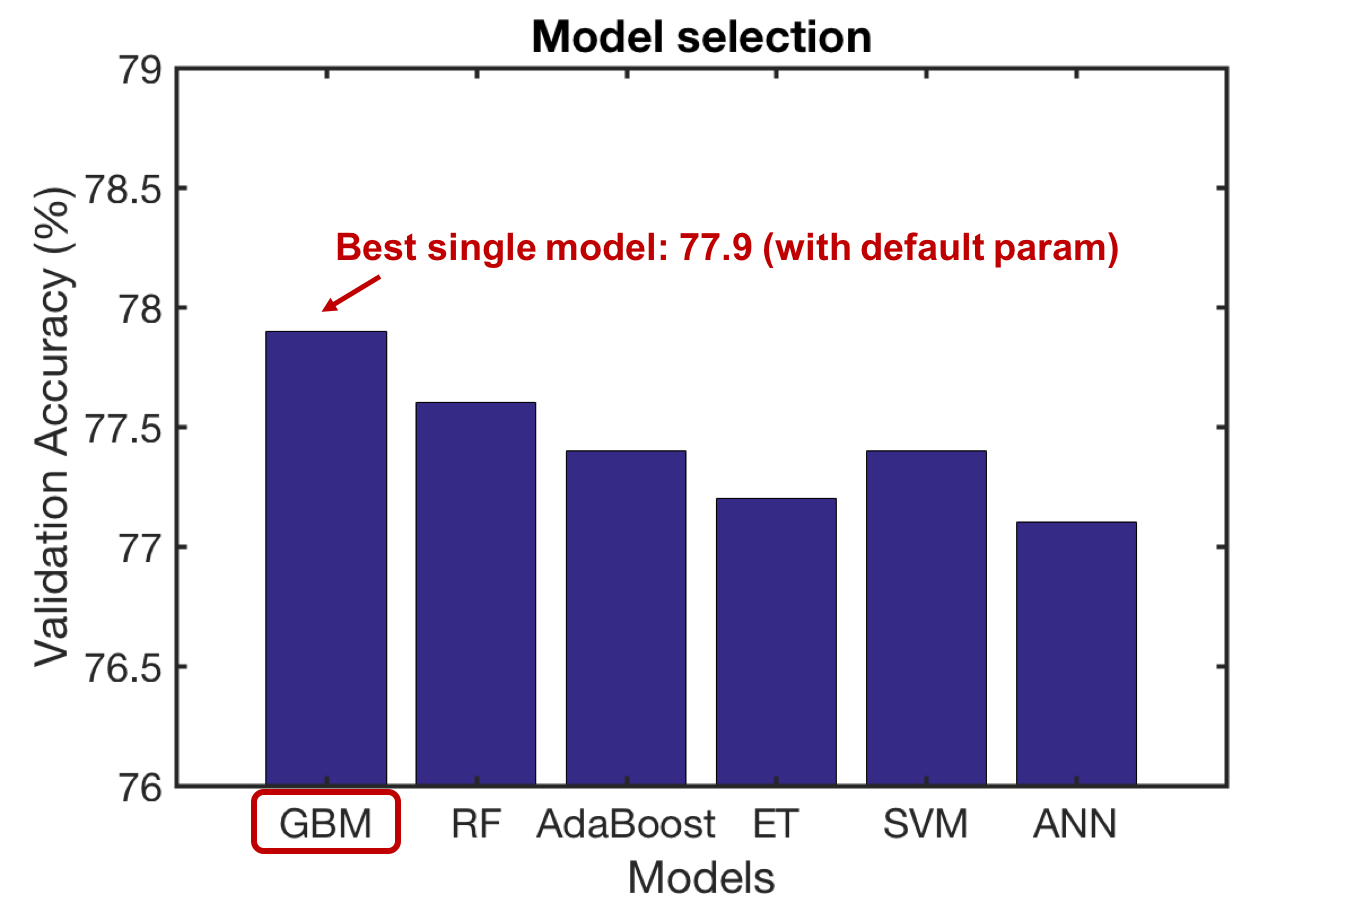
\includegraphics[scale=0.45]{figure2/figure2.png}
\caption{\textbf{Cross validation for single best model selection} \textit{GBM attains the highest accuracy of $77.9\%$ followed by random forests(77.6), Adaboost(77.4), Extra Trees(77.2), Support Vector Machines (77.4), and Artificial Neural Networks (77.1).}}
\end{figure}

Generally, we saw that tree-based non-linear classifiers out-performed linear models such as support vector machines. We attribute this to the fact that demographic features are often only separable by highly non-linear discriminant boundaries. This is in agreement with the fact that the training data projected onto the first two principal components showed no notable separating boundaries. (Hence, our attempt to preprocess the data using principal component eigenvector bases transformation was unsuccessful) This influenced our decision of including more tree-based non-linear classifiers into the pool of models to perform cross validation on. GBMs proved to be a low variance model as it achieved repeatable validation accuracy. (Random forests had relatively higher variance) However, the low variance characteristic made it difficult to enhance the performance of GBMs by only including GBMs in the pool of trained models to ensemble select on. Section 3.3-[iii] will elaborate more on this issue. We now move on to show the results of optimizing GBM model parameters. 

\newpage

\subsubsection*{[ii]. Parameter optimization for GBM}
After selecting Gradient Boosting Machines(GBM) as the single best model, we sought to optimize the boosting base model (decision tree) parameters as well as the boosting specific parameters. We considered 5 main parameters for optimization: minimum leaf size, maximum height, learning rate, subsample, and number of estimators. Minimum leaf size and maximum height are both decision tree parameters which control the degree of regularization. Moreover, learning rate, subsample, and number of estimators alters the degree of stochasticity in training each base model, the constants involved in the boosting equation, and the number of boosted trees to train. The number of estimators demonstrated no significant impact on the cross validation accuracy beyond 500 trees and thus we omit the plot regarding this parameter. In fig. 4. we show the validation accuracy of the GBM model plotted against the remaining 4 parameters subject to optimization. The optimum parameters were discovered through a grid search function provided by sklearn, which performs cross validation on the full space of possible parameter quadruples (min leaf size, max height, learning rate, sub sample). Here we show the cross validation performance of each parameter separately, while fixing all other parameters to be the optimum values. Due to the slight randomness in the model that the learning algorithm converges to, the maximum cross validation accuracy differs slightly from plot to plot. Since we seek to show quantitative rationale for our choice of the optimum parameters, we deem these plots as sufficient. The overall best parameters chosen for the GBM model were: (min leaf size, max height, learning rate, sub sample) = (15, 3, 0.1, 1). 
\begin{figure}[h]
\center
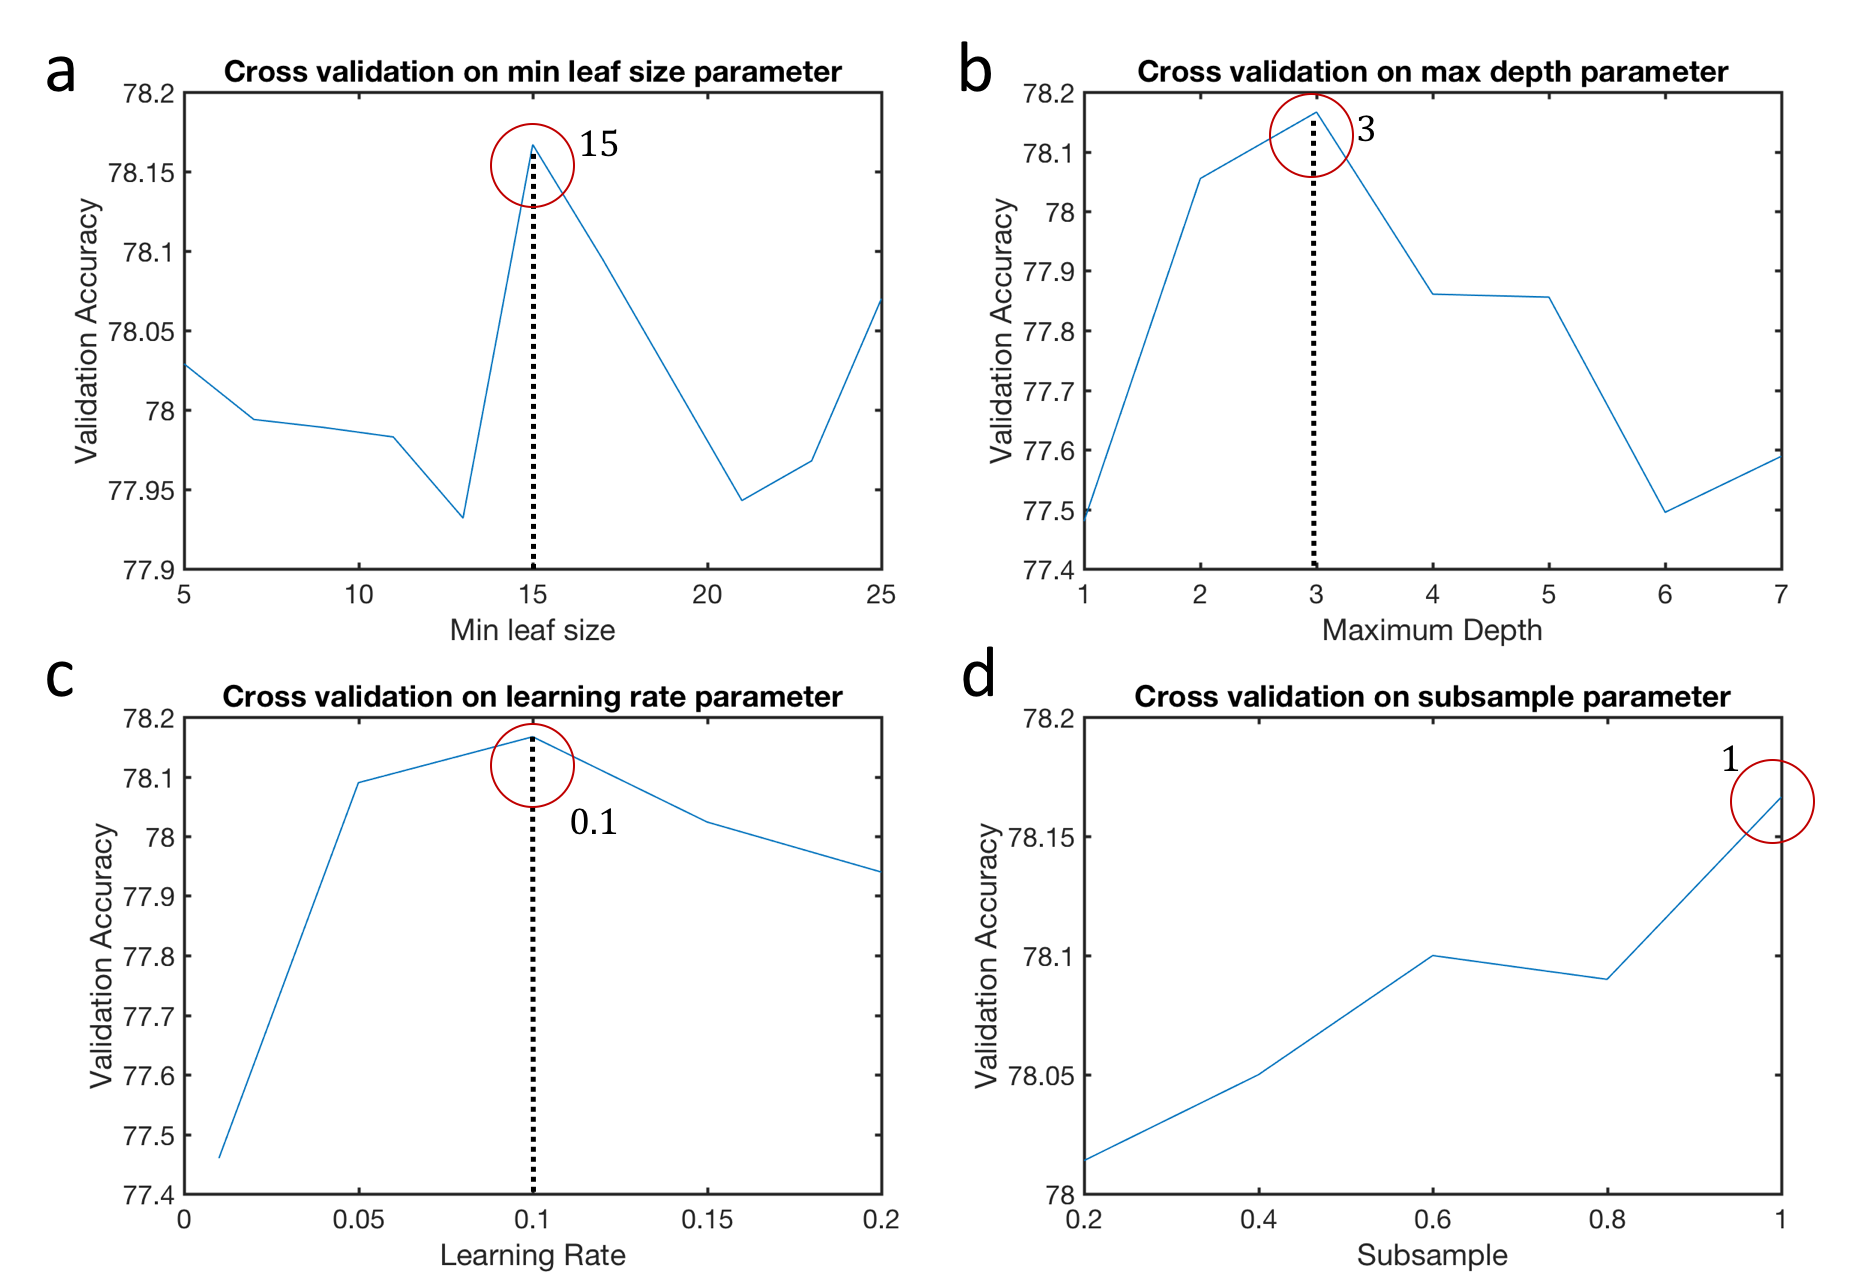
\includegraphics[scale=0.4]{figure3/figure3.png}
\caption{\textbf{Cross validation for model parameter selection} \textit{Through an exhaustive grid search we determined the quadruple of parameters which gave the best validation accuracy around $78.2\%$. (a) Validation on min leaf size shows a peak at 15 (b) Validation on max depth shows peak at 3 (c) Validation on learning rate shows a peak at 0.1 (d) Validation on subsample shows a peak at 1}}
\end{figure}


\newpage
\subsubsection*{[iii]. Handling class-imbalance}
Upon analyzing the label distribution of the training data, we found that over $73\%$ were of class $1$, while only $27\%$ were class 2. Such class-imbalance can often lead to the tree predicting in favor of the majority class, which generates a low-precision, high-recall classifier. (In terms of the majority class) Our solution to tackling this class-imbalance problem was to set a prediction bias. To elaborate, first recall that a decision tree makes predictions by taking the argmax of the probability distribution over the class-labels at each leaf node. For a binary classification task, this means that the class with probability higher than 0.5 becomes the prediction. We instead modify the threshold with a prediction bias $p$ such that in order for class 1 to be the prediction at a leaf node, it must have a probability $0.5 + p$. Fig. 4. shows cross validation accuracy while varying $p$ from $-0.02$ to $0.02$. Other bias values ($> 0.2$ or $< -0.2$) led to worse model performance than the optimum value $p = 0.013$. 
\begin{figure}[h]
\center
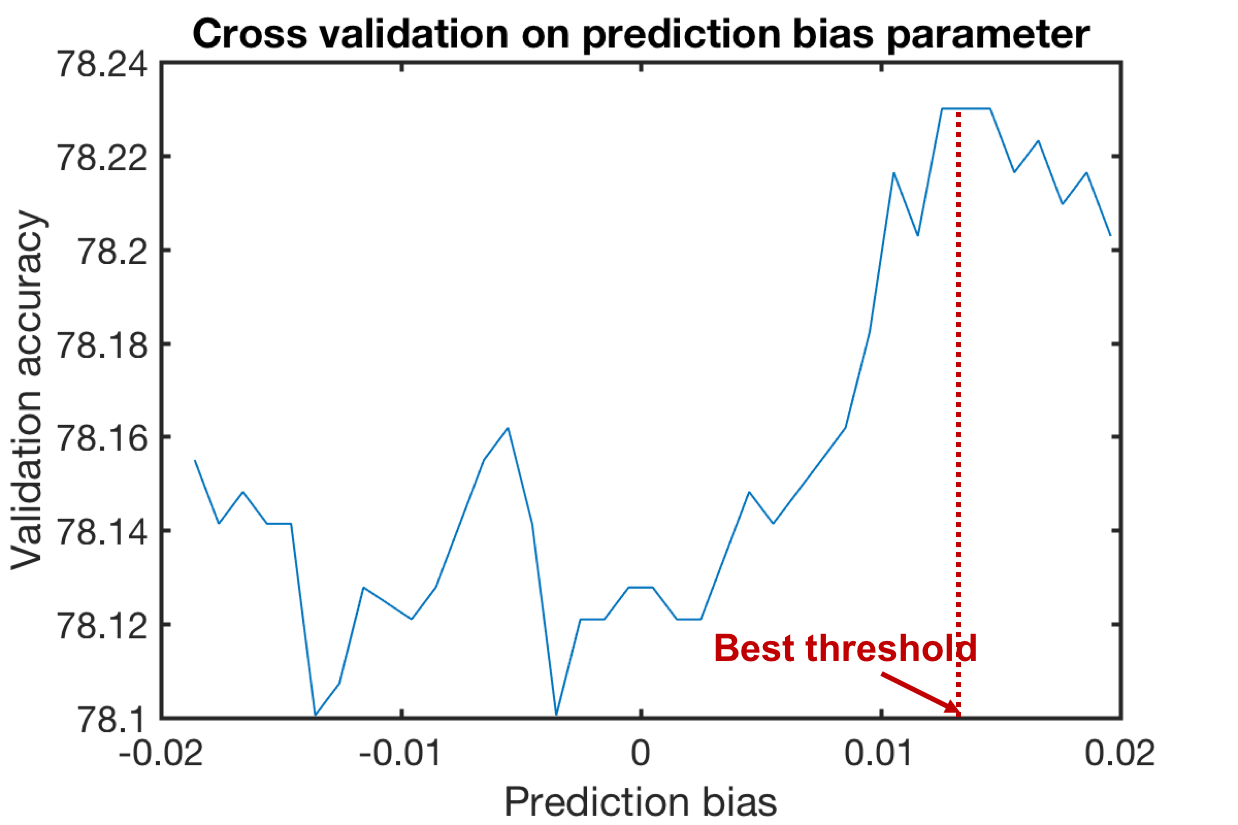
\includegraphics[scale=0.5]{figure4/figure4.png}
\caption{\textbf{Cross validation accuracy vs prediction bias} \textit{Validation accuracy is highest with a prediction bias of $0.013$. Qualitatively, a positive prediction bias means to predict in favor of class 2 (minority class). }}
\end{figure}

\subsubsection*{[iv]. Ensemble selection}
$85\%$ of the total training data was partitioned towards training a model library and $15\%$ was reserved as a validation set to ensemble select on. We trained a model library consisting of $20$ GBMs, $20$ ANNs, and $20$ Random Forests. Upon an initial attempt of building a library with only GBMs, we realized that boosting methods have very low variance. Hence, most models generated similar predictions and ensemble selection did not lead to an improvement in the validation accuracy. Hence, we decided to add more diverse models into the pool in order to take the full benefit of both bagging and boosting. For succinctness of the report, we omit the parameter optimization process for ANNs and RFs. The final accuracy of the ensemble selected model was approximately $0.1$ better than a single GBM attaining the highest validation accuracy $\approx 78.3$. Our submission of this model received a \textbf{final score of 78.7 on the 2008 dataset and 76.17 on the 2012 dataset}. 

\newpage

\section*{4. Conclusion}
\subsubsection*{[i]. Overall rank: $9^{th}$ for 2008 dataset, $26^{th}$ for 2012 dataset}
\subsubsection*{[ii]. Discoveries}


\subsubsection*{[iii]. Challenges}
Dealing with real-word data was more difficult than training models to fit low-noise data which are often given out for homework assignments. We believe that learning how to engineer the features effectively was the most challenging aspect of this project. This required us to understand the features beyond their numeric values, which required many hours because there were 380 of them. We learned that many feature engineering techniques are task specific which led to many of our initial attempts (such as PCA, Univariate selection) failing. As a more concrete example, it was difficult to decide what to do with the various nonresponse values (negative values), as described in Section 3.2. Ensuring that the transformed training data and test data were compatible (ie, had the same shape) was an issue because our handling of categorical features sometimes created discrepancies in the number of features between the training and test sets. For instance, that a categorical feature attains values 1 and 2 in the training set and 3 in the test set. Then the transformed training set will have two features for the original categorical feature, whereas the transformed test set will have only one. This was remedied by adding additional feature columns to both data sets to ensure that they had the same features. Through overcoming these challenges, the most important lesson that we learned was that it is crucial to fully understand the data before attempting any feature selection or model optimization. 

\subsubsection*{[iv]. Concluding Remarks}
This competition gave us a sense of the difficulties machine learning practitioners face when modeling noisy real-word data. Lastly and most importantly, we would like to thank the TAs and the instructor for organizing such a great learning experience. We hope our report demonstrates that your efforts to find creative ways in teaching were not in vein. 

















\end{document}